\section{Anexo}\label{sec:anexo}

\subsection{Anexo 1: Repositorio abierto del trabajo}\label{anexo1:repo}
Para este trabajo final se utilizó la herramienta de control de versionado GIT, puntualmente alojado en la plataforma GitHub, y el tanto el código como los modelos generados por este trabajo son abiertos, es decir, cualquier persona puede acceder y hacer uso de lo realizado bajo su propia responsabilidad (ver Licencia del proyecto \ref{anexo2:license}). Además, la estructura de los directorios elegida se detalla a continuación:
\begin{itemize}
	\item LICENSE: Licencia del proyecto.
	\item README.md: Archivo de lectura inicial para desarrolladores o quien esté interesado en conocer el proyecto.
	\item data: directorio con los conjuntos de datos.
		\subitem - external: bancos de datos comprimidos.
		\subitem - interim: conjuntos de datos utilizados en cada experimento comprimidos.
		\subitem - processed: directorios con conjuntos de datos finales para entrenar y medir rendimiento de modelos (divididos en conjuntos de entrenamiento, validación y verificación cada uno).
		\subitem - raw: bancos de datos en crudo (sin dividir en conjuntos diferentes).
	\item docs: directorio con el presente documento, tanto en su versión compilable LaTex como en PDF.
	\item models: directorio con los modelos entrenados, instancias de abstracciones propias creadas y archivos json con los pesos de las redes entrenadas.
	\item notebooks: directorio con Jupyter Notebooks versionados con los que se trabajó durante el proyecto.
	\item requirements.txt: archivo con librerías requeridas para poder ejecutar correctamente el contenido del repositorio.
	\item setup.py: archivo de instalación del repositorio para poder importarlo como una librería python.
	\item src: directorio con el código fuente utilizado en el proyecto.
		\subitem - data: módulos utilizados para generar los diferentes conjuntos de datos.
		\subitem - models: módulos con las abstracciones utilizadas para entrenar y medir el rendimiento de los modelos.
		\subitem - visualization: módulos con visualizaciones.
\end{itemize}

\subsection{Anexo 2: Licencia del proyecto}\label{anexo2:license}
La licencia del presente proyecto es la \(Licencia\) \(MIT\) (en su versión \(X11\)), es para software libre de código abierto y especifica lo siguiente:
\begin{enumerate}
	\item Condiciones: La condición es que la nota de copyright y la parte de los derechos se incluya en todas las copias o partes sustanciales del Software. Esta es la condición que invalidaría la licencia en caso de no cumplirse.
	\item Derechos: sin restricciones; incluyendo usar, copiar, modificar, integrar con otro Software, publicar, sublicenciar o vender copias del Software, y además permitir a las personas a las que se les entregue el Software hacer lo mismo.
	\item Limitación de responsabilidad: finalmente se tiene un disclaimer o nota de limitación de la responsabilidad habitual en este tipo de licencias.
\end{enumerate}

\subsection{Anexo 3: Mapeo de clases realizado para el experimento \ref{sssec:exp3}}\label{ssec:anexo3}
En la tabla \ref{anexo:exp3:mapping} se presentan los mapeos elegidos entre las clases con las que la red PlacesCNN fue entrenada y las clases esperadas que se predigan para el dataset utilizado en el experimento \ref{sssec:exp3}.
\begin{table}[h!]
	\noindent
	\begin{tabular}{||l|l||l|l||}
		\toprule                                                                                        		Clase en Places365 &       Mapeo & 		Clase en Places365 &       Mapeo \\                                                                                                       
		\midrule
		\midrule 
		apartment\_ &    {} &       hospital\_room &     bedroom \\
		building/outdoor &    frontyard &       {} &     {} \\
		\midrule                                                                                 
		bathroom &     bathroom &          hotel\_room &     bedroom \\
		\midrule
		bedchamber &      bedroom &               house &   frontyard \\
		\midrule                                                                                   
		bedroom &      bedroom &              kasbah &   frontyard \\      
		\midrule                                                                              
		building\_facade &    frontyard &             kitchen &     kitchen \\
		\midrule
		chalet &    frontyard &        lecture\_room &  livingRoom \\
		\midrule
		childs\_room &      bedroom &         living\_room &  livingRoom \\
		\midrule
		clean\_room &      bedroom &               lobby &  livingRoom \\
		\midrule
		closet &      bedroom &   manufactured\_home &   frontyard \\
		\midrule
		cottage &    frontyard &     office\_cubicles &  livingRoom \\
		\midrule
		courthouse &    frontyard &               patio &   frontyard \\
		\midrule
		courtyard &    frontyard &               porch &   frontyard \\
		\midrule
		diner/outdoor &  dining\_room &     recreation\_room &  livingRoom \\
		\midrule
		dining\_hall &  dining\_room &  restaurant\_kitchen &     kitchen \\
		\midrule
		dining\_room &  dining\_room &              shower &    bathroom \\
		\midrule
		doorway/outdoor &    frontyard &     television\_room &  livingRoom \\
		\midrule
		dorm\_room &      bedroom &   television\_studio &  livingRoom \\
		\midrule
		dressing\_room &      bedroom &        waiting\_room &  livingRoom \\
		\midrule
		home\_office &   livingRoom &                yard &   frontyard \\
		\midrule
		home\_theater &  livingRoom & & \\
		\bottomrule
	\end{tabular}
	\caption{Mapeo entre clases con las que la red PlacesCNN fue entrenada y las clases del conjunto de datos utilizado en el experimento \ref{sssec:exp3}}
\label{anexo:exp3:mapping}
\end{table}



\subsection{Anexo 4: Arquitectura del Perceptrón Multicapa utilizado en experimento \ref{sssec:exp1}}\label{ssec:anexo4}
\begin{figure}[h!]
\centering
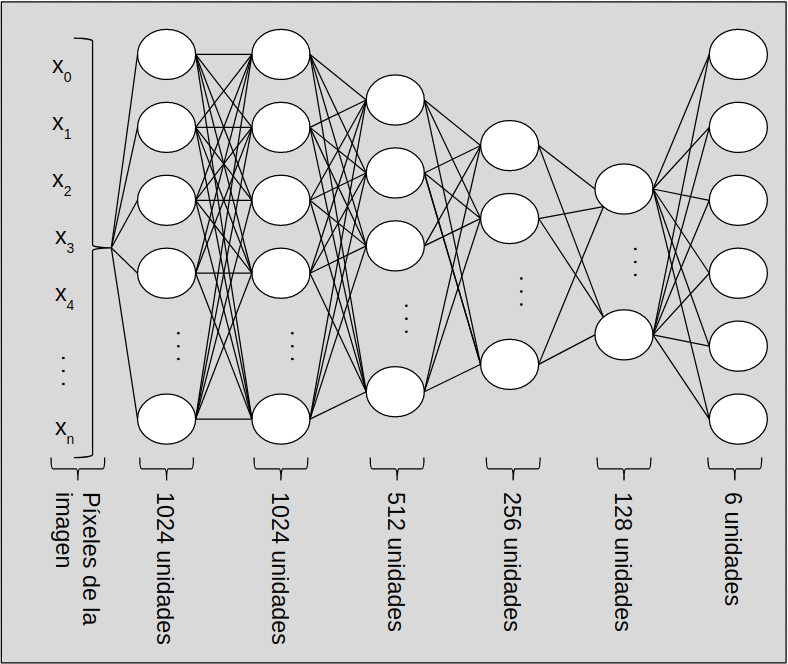
\includegraphics[width=0.7\linewidth]{images/architecture_exp1}
\caption{Arquitectura perceptrón multicapa del experimento \ref{sssec:exp1}}
\label{fig:architectureexp1}
\end{figure}


\subsection{Anexo 5: Arquitectura de la Red Neuronal Convolucional utilizada en los experimentos \ref{sssec:exp1} y \ref{sssec:exp2}}\label{ssec:anexo5}

\begin{figure}[h!]
	\centering
	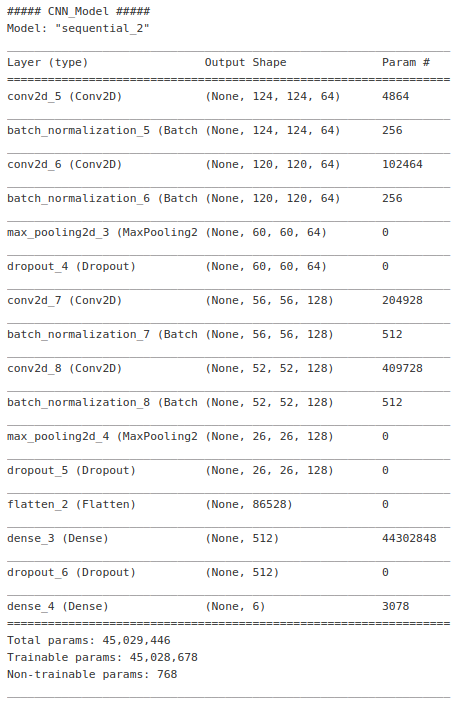
\includegraphics[width=0.7\linewidth]{images/architecture_exp1_cnn}
	\caption{Arquitectura Red Neuronal Convolucional de los experimentos \ref{sssec:exp1} y \ref{sssec:exp2}}
	\label{fig:architectureexp2}
\end{figure}


\subsection{Anexo 6: Arquitectura de la red PlacesCNN utilizada en experimento \ref{sssec:exp3}}\label{ssec:anexo6}

\begin{figure}[h!]
	\centering
	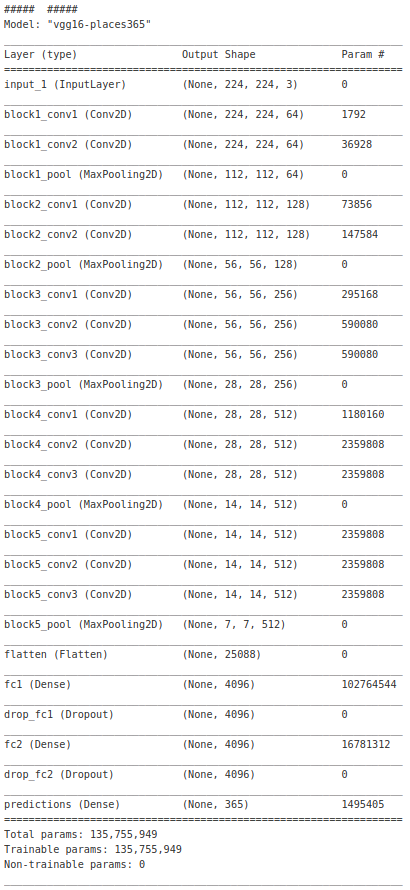
\includegraphics[width=0.7\linewidth]{images/architecture_exp3}
	\caption{Arquitectura Red Neuronal Convolucional del experimento \ref{sssec:exp3}}
	\label{fig:architectureexp3}
\end{figure}


\subsection{Anexo 7: Arquitectura utilizada en experimentos \ref{sssec:exp4} y \ref{sssec:exp6}}\label{ssec:anexo7}

\begin{figure}[h!]
	\centering
	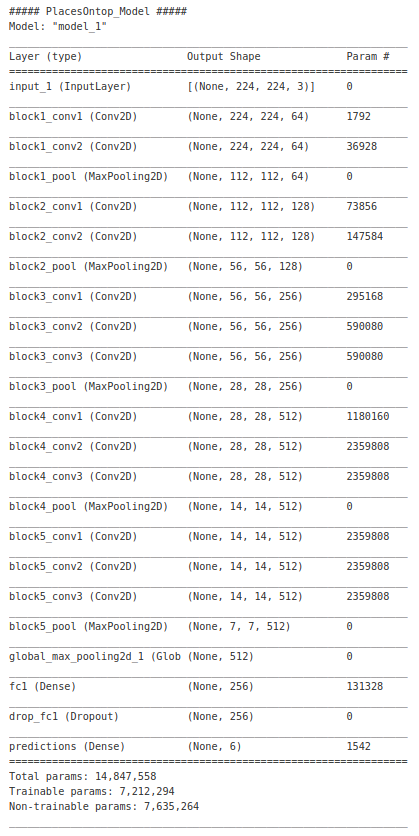
\includegraphics[width=0.7\linewidth]{images/architecture_exp4_6_cnn}
	\caption{Arquitectura Red Neuronal Convolucional de los experimentos \ref{sssec:exp4} y \ref{sssec:exp6} }
	\label{fig:architectureexp4_6}
\end{figure}


\subsection{Anexo 8: Arquitectura utilizada en experimento \ref{sssec:exp5}}\label{ssec:anexo8}

\begin{figure}[h!]
	\centering
	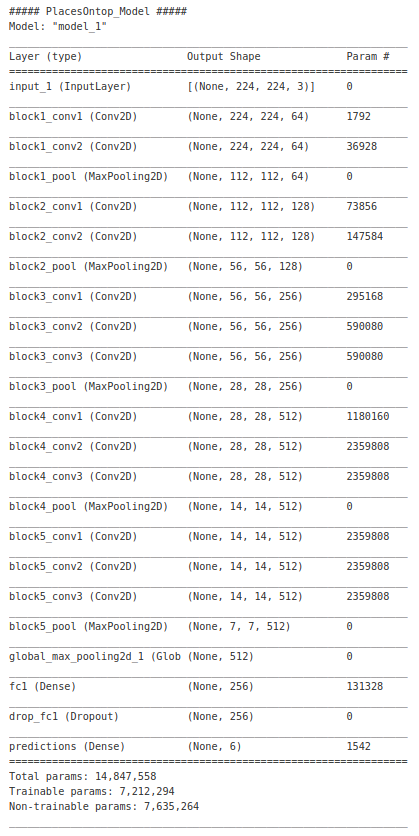
\includegraphics[width=0.7\linewidth]{images/architecture_exp4_6_cnn}
	\caption{Arquitectura Red Neuronal Convolucional del  experimento \ref{sssec:exp5}}
	\label{fig:architectureexp5}
\end{figure}